\documentclass{beamer}

\usepackage{amsmath}
\usepackage{amssymb}
\usepackage{amsthm}
\usepackage{mathtools}
\usepackage[UKenglish]{babel}
\usepackage{enumerate}
\usepackage{graphicx}
\usepackage{braket}
\usepackage{esint}
\usepackage{float}
\usepackage{tabularx}
\usepackage{array}
\usepackage{subcaption}
\usepackage{hyperref}
\usepackage{xcolor}
\hypersetup{colorlinks=false, bookmarks=true}


\usetheme{Madrid}
\usecolortheme{seahorse}
\usefonttheme{professionalfonts}
\useinnertheme{circles}

\AtBeginSection[]
{
  \begin{frame}
    \frametitle{Table of Contents}
    \tableofcontents[currentsection]
  \end{frame}
}

\setbeamertemplate{caption}[numbered]

\title[QCNN State Preparation]{A QCNN for Quantum State Preparation}
\subtitle{Carnegie Vacation Scholarship}
\author[David Amorim]{David Amorim}
\institute[]{}
\date[21/08/2024]{Weeks 7-8 \\(12/08/2024 - 23/08/2024)}

\begin{document}

\frame{\titlepage}

\begin{frame}
\frametitle{Aims for the Week}
The following aims were set at the last meeting (14/08/2024):

\begin{alertblock}{New Phase Encoding Approach}
Investigate a new approach to phase encoding using linear piecewise phase functions without explicit function evaluation.  
\end{alertblock}

\begin{alertblock}{Handover}
Hand over the slides, documentation, code and the poster for the Carnegie Trust.
\end{alertblock}
\end{frame}

\section{Phase Encoding}

\begin{frame}
\frametitle{Preliminaries}

\begin{itemize}
\item Consider an \alert{$n$-qubit} register with computational basis states $\ket{j} = \ket{j_0 j_1 ... j_{n-1}}$ representing $n$-bit strings
\item Let \alert{$p$} of the register qubits be \alert{precision qubits} so that 
\begin{equation}
j = \sum^{n -1}_{k=0} j_k 2^{k-p}
\end{equation} 
\item Consider a \alert{phase function} $\Psi$ over the domain $\Omega = \{ j \}$ and construct an \alert{$M$-fold partition} ($M = 2^g$, $g \leq n \in \mathbb{N}$) into equal sub-domains $\Omega_m$:
\begin{equation}
\Omega = \bigcup_{m=1}^M \Omega_m, \; \; \; \Omega_m \cap \Omega_l = \emptyset, \;  \; \; |\Omega_m| = |\Omega_l|
\end{equation}
\item On each sub-domain, approximate $\Psi$ using a \alert{linear function}:
\begin{equation}
\Psi(j) = \alpha_m j + \beta_m, \; \; \; j \in \Omega_m
\end{equation}
\end{itemize}

\end{frame}

\begin{frame}

\frametitle{Phase Encoding within a Sub-domain}

\begin{block}{Aim 1}
For $j \in \Omega_m$ construct an operator $\hat{O}_m$ such that $\ket{j} \mapsto e^{i (\alpha_m j + \beta_m )} \ket{j}$. 
\end{block}

\begin{itemize}
\item Consider the single-qubit operators 
\begin{equation}
\hat{P}^{(k)}(\varphi) = \begin{pmatrix}
e^{i \varphi} & 0 \\ 0 & e^{i \varphi}
\end{pmatrix}, \; \; \; \hat{R}^{(k)}(\varphi) = \begin{pmatrix}
1 & 0 \\ 0 & e^{i \varphi}
\end{pmatrix}
\end{equation}
each acting on the $k$th qubit
\item Then 
\begin{equation}
\hat{O}_m \equiv \bigotimes^{n-1}_{k=0} \hat{P}^{(k)} (\beta_m / n) \hat{R}^{(k)} \left( \alpha_m 2^{k-p} \right)
\end{equation}
transforms 
\begin{equation}
\ket{j} \mapsto \exp \left[ i \left( \sum_{k=0}^{n-1} \alpha_m j_k 2^{k-p} + \beta_m \right) \right] \ket{j} = e^{i (\alpha_m j + \beta_m )} \ket{j}
\end{equation}
\end{itemize}
\end{frame}

\begin{frame}
\frametitle{Selecting the Subdomain}
\begin{itemize}
\item It is straight-forward to construct $\hat{O}_m$ for each of the sub-domains $\Omega_m$ 
\item More challenging is applying the correct $\hat{O}_m$ based on the sub-domain corresponding to each $\ket{j}$
\end{itemize}
\begin{block}{Aim 2}
Construct a system of controls such that $\hat{O}_m$ is applied to $\ket{j}$ if and only if $j \in \Omega_m$
\end{block}
\end{frame}

\begin{frame}
\frametitle{Sample Case: $M=2$}
\begin{columns}
\begin{column}{0.4\textwidth}
\begin{itemize}
\item Start with the simplest possible case, a 2-fold partition ($M=2$): 
\begin{equation}
j \in \begin{cases}
\Omega_1 & j_0 = 0 \\
\Omega_2 & j_0 = 1
\end{cases}
\end{equation}
\item Using an ancilla qubit, $\hat{O}_1$ is applied for $j \in \Omega_1$ and $\hat{O}_2$ for $j \in \Omega_2$
\item The ancilla is required since the operation applied to $\ket{j_0}$ is conditional on $\ket{j_0}$ itself 
\end{itemize}
\end{column}
\begin{column}{0.6\textwidth}
\begin{figure}
\centering 
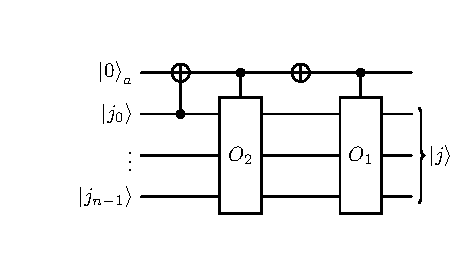
\includegraphics[width=\textwidth]{im/circuit_2-fold}
\caption{Circuit diagram for $M=2$}
\end{figure}
\end{column}
\end{columns}
\end{frame}

\begin{frame}
\frametitle{Generalising the Approach}
\begin{columns}
\begin{column}{0.4\textwidth}
\begin{itemize}
\item The approach shown on the previous slide requires $1 \leq  \log_2 M  \leq n $ ancilla qubits
\item The number of controls required is $\sim \mathcal{O}(M \log M)$ as there are $M$ operators, each controlled by all ancillas 
\item A `pyramid' network of X gates is applied to the ancillas for case distinction
\item For $M \sim 2^n$ the gate cost is exponential!
\end{itemize}
\end{column}
\begin{column}{0.6\textwidth}
\begin{figure}
\centering
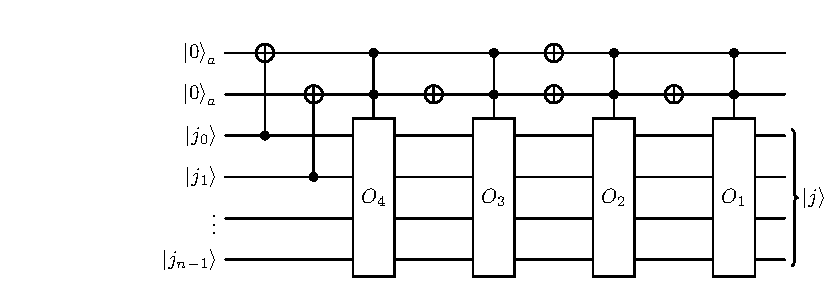
\includegraphics[width=\textwidth]{im/circuit_4-fold}
\caption{Circuit diagram for $M=4$. Note that $j \in \Omega_m$ if $j_0j_1 =m-1$ (e.g. $j\in \Omega_3$ if $j_0 j_1 =10$ ).}
\end{figure}
\end{column}
\end{columns}
\end{frame}

\begin{frame}
\frametitle{A Recursive Approach}
\begin{itemize}
\item Since $M=2^g$ for some $g \leq n \in \mathbb{N}$ we can view the partition of $\Omega$ as a recursive process, splitting the domain into halves $g$ times
\item ....
\end{itemize}

TRY TO GET RID OF ANCILLAS!! THIS IS ESSENTIALLY A CLASSICAL ALGORITHM! MUST BE POSSIBLE TO DO IT BETTER!!
\end{frame}

\begin{frame}
\frametitle{Qiskit Implementation}


\end{frame}



\section{Handover}

\begin{frame}

\frametitle{Handover}

The code, documentation, slides, and poster are all available on GitHub:
\begin{center}
\vspace{0.6cm}
\href{https://github.com/david-f-amorim/PQC_function_evaluation}{\texttt{https://github.com/david-f-amorim/PQC\_function\_evaluation}}
\vspace{0.6cm}
\end{center}

\begin{itemize}
\item The source code is found in the directory \alert{\texttt{pqcprep}} 
\item The slides and poster are found in the directory \alert{\texttt{slides}}
\item The documentation is hosted externally  \href{https://david-f-amorim.github.io/PQC_function_evaluation/pqcprep.html}{\textcolor{purple}{here}}, which is linked on GitHub
\end{itemize}

\end{frame}

\end{document}